
\section{Background}\label{sec:background}






\subsection{Computational Thinking}
Computational Thinking (CT) was coined in 2006 by Wing and considered the extension of every child's analytical ability (\cite{Wing2006}). CT refers to thought processes that are involved when solving complex problems and generalizing and transferring this problem solving process to a wide variety of problems (\cite{voogt2015computational}). CT are higher-order-thinking skills  (\cite{Yadav2017CTteacherEd}).



There is no general consensus on the definition of Computational Thinking (\cite{Yadav2015}). Voogt et al. (\cite{voogt2015computational}) call for a flexible and pragmatic approach and use operationalization of CT, such as has been done by Yadav (\cite{Yadav2015}). Selby and Woollard (\cite{selby2013computational}) sought a narrower definition to facilitate assessment. They tallied occurring terms, descriptions, and meanings for CT in different definitions found in literature. Then, considering the motivation by each individual author for either incorporating or neglecting the term, they came to ordered criteria, which do not necessarily to accommodate alle viewpoints. Selby and Woollard describe Computational Thinking as a focused approach to problem solving, incorporating thought processes that utilize \emph{abstraction}, \emph{decomposition}, \emph{algorithmic design}, \emph{evaluation}, and \emph{generalizations}.
%
%\begin{itemize}
%\item Algorithmic Thinking: thinking in terms of rules, steps and repetitions (of subtasks).
%\item Decomposition: Breaking a problem into sub-problems (which can be dealt with individually).
%\item Abstraction: simplifying a problem by leaving out (irrelevant) details.
%\item Generalization: finding patterns and re-using solutions (transfer).
%\item Evaluation: Does my solution solve the problem? Analysis: How could process/solution have been improved?
%\item Automation: implementation (through computing tools).
%\end{itemize}

Corradini et al. (\cite{corradini2017conceptions}
compared and analyzed five well-cited definitions (Wing \cite{Wing2006}, CSTA\cite{CSTA2011CT}, Google\cite{Google2017CT}, Brennan and Resnick\cite{BrennanResnick2012}, and Barefoot CAS\cite{CAS2014CT}) to come to common grounds. They grouped common aspects to four categories:
\begin{itemize}
\item mental processes (algorithmic thinking, logical thinking, decomposition, abstraction, pattern recognition, generalisation)
\item methods (automation, data collection, analysis and representation, parallelization, simulation, evaluation and programming)
\item practices (experimenting, iterating, tinkering, testing, debugging, reusing, remixing)
\item transversal skills (create, communicate, collaborate, reflect, learn, meta-reflect, and be tolerant for ambiguity).
\end{itemize}

The approaches and attitudes from CAS and CSTA definitions also coincide with the Skills domain in the reformed curriculum. Common aspects are designing, developing, collaborating and communicating. Attitudes, such as CSTA's mindset to deal with open ended problems, complexity and tolerance for ambiguity are not mentioned specifically but are pre-requisite to the abilities that are explicably mentioned (such as "to weigh the options of a digital artefact by means of research and experimentation").



\subsubsection{CT and programming}

Several studies report an evident link between programming and CT. In his analysis Hu \cite{hu2011computational} state that developing computational thinking skills would make students better prepared and more successful in learning programming. However, IT devices are not absolutely needed to develop CT competencies in students\cite{corradini2017conceptions}. Davies et al. (\cite{davies2008effects}) focus on teaching CT skills prior to a programming language, and conclude that such an approach enhances programming skills.

In the reverse direction, Yadav \cite{Yadav2017CTteacherEd} expresses that creating computational artifacts increases creative expression and thus problem solving skills. Brennan and Resnick (\cite{BrennanResnick2012}) use programming to develop computational thinking. And in their review study, Lye and Koh (\cite{LyeKoh2014}) analyse different ways of exposing students to computational thinking through programming.


In his article, Denning \cite{denning2017remaining} differentiates between traditional CT (prior to the 2006 Wing 'movement') and new CT. Where in the traditional CT, programming ability is described to produce CT, and in the new, CT is a conceptual framework that enables programming. In the new CT, Programs are loosely coupled with algorithms and translation it into a program is optional. The solution of the problem must be expressed precisely and unambiguously in a way that a processing agent can carry it out, but for all that matters, that processing agent can be either a human or a machine\cite{corradini2017conceptions}.

What is important to take away from this discussion, is that there is a fundamental difference between CT and programming. CT encompasses the design of an algorithm. A flowchart could be used to articulate and visualize an algorithm. Programming pertains to implementation, using concepts and constructs of a programming language to translate the algorithm into code and creating a digital artefact. So, CT and programming require different skills, and assessment should be based using evidence from different outputs.

%In a survey of program understanding, von Mayrhauser and Vans
%(1994) summarise studies (in particular Guindon, 1990) noting that experts:
%have efficiently organised and specialised knowledge schemas; organise their
%knowledge according to functional characteristics such as the nature of the
%underlying algorithm (rather than superficial details such as language syntax);
%use both general problem solving strategies (such as divide-and-conquer) and
%specialised strategies; use specialised schemas and a top-down, breadth-first
%approach to efficiently decompose and understand programs; and are flexible in their approach to program comprehension and their willingness to abandon
%questionable hypotheses.[Robins, Rountree, Rountre (2003).  ]


\subsection{Algorithms, Algorithmic Thinking, and Problem Solving}


Wing \cite{Wing2006}describes CT as a linking pin in CS: "solving problems, designing systems, and understanding human behavior, by drawing on the concepts fundamental to computer science". ISTE and CSTA define CT as "a problem-solving process"\cite{CSTA2011CT} and characterize it as "automating solutions through algorithmic thinking". The reformed curriculum refers to computational thinking and problem solving in the \emph{Using informatics as a perspective} sub-domain: "analytical skills to formulate problems in such a way that one can use computers and other tools to help solve them, as well as problem solving skills,
such as finding solutions in terms of algorithms and data"\cite{Barendsen2016}. This coincides with the ISTE-CSTA definition.



Algorithms are a fundamental CS concept. Algorithms are tools for developing and expressing solutions to computational problems (\cite{GroverPea2013}). Based on the CT definitions from \cite{CAS2014CT}, \cite{Google2017CT},\cite{BrennanResnick2012} and \cite{CSTA2011CT}, Algorithmic thinking is the process of designing a sequence of ordered steps (instructions) to solve a problem, achieve a goal or perform a task\cite{corradini2017conceptions}. To be successful in developing novel algorithms that solve problems correctly and successfully, calls for a coherent set of skills and knowledge. On the one hand, algorithmic thinking (as part of CT) and problem-solving skills are essential for programming, and thus developing algorithms(\cite{McCracken2001}). On the other, fundamental knowledge of the concepts of algorithms are needed, i.e., how algorithms work, which common algorithms and plans exist, and knowledge about strategies for composing (or combining) algorithmic components (\cite{deRaadt2008}). CT thought processes are involved in formulating problems so their solutions can be represented as computational steps and algorithms (\cite{aho2012computation}). In 1974, Donald Knuth said that articulating a solution as an algorithm and implementing (and testing) the concept on a computer leads to a deep understanding of concepts of all kinds in many fields.




\todo{How to develop skills and reinforce knowledge related to algorithms… either through concepts or programming. <SEE VERHAAL VAN DENNING, 2017>}


McCracken et al. (\cite{McCracken2001}) describe five iterative steps to problem solving (abstracting, generating sub-problems, implementing sub-solutions, integrating sub-solutions, evaluating and iterating). These steps encompass the CT skills (algorithmic thinking, abstraction, decomposition, generalization, evaluation) as described by Wing (2006). The step of integrating sub-solutions (via abutment, merging and nesting) corresponds with algorithmic thinking, as it involves creating an algorithm that controls the sequence of events. An important aspect of the reverse step, generating sub-problems, is recognizing plans, existing methods or strategies. Recognizing plans at an abstract level helps decompose the problem and simplifies reasoning about its solution (\cite{Smetsers2017}). What remains is to fine-tune the plan to the specific situation and then integrate it with the remaining sub-solutions.


\subsection{Assessment and criteria}


Assessments are used for several purposes. McMillan (\cite{mcmillan2007formative}) distinguishes between two types of assessments, summative and formative. Summative assessment refers to the use of assessment-based evidence to help us arrive at go/no-go decisions based on the success of a completed course or instructional program (\cite{popham2009assessment}). On the other hand, assessment for learning is formative. Formative assessment is used by both students and teachers to adjust ongoing instructional and learning activities in order to improve the manner in which learning is taking place. Summative assessment can also be treated formatively, for example to determine the effectiveness of instruction.




A substantial amount of research has been done into the role of assessment in education. In his study Frederiksen (\cite{frederiksen1984}) describe assessment as a motivator for learning. Alderson and Wall (1993) and Prodromou (1996) elaborate by stating that what is assessed strongly influences what is learned. Biggs (\cite{biggs1996}) prescribes that instruction, learning and assessment must be well-aligned. This alignment exists in most traditional knowledge-based tests, yet constructive alignment for competency-based instruction is not self-evident (\cite{baartman2006wheel}). With the emphasis of Computational Thinking and problem solving in reformed CS curricula, learning and instruction is increasingly competency-based. Assessment of competencies is complex, mainly because it comprises a multi-facetted blend of knowledge, skills and attitudes (\cite{merrienboer2002competenties}). CT is a skill and this tacit knowledge should be assessed directly\cite{denning2017remaining}. Assessment should thus elicit behaviors which indicate that a student can master the competency. As Denning formulates it: "\emph{given that so much education is formulated around students acquiring knowledge, looking carefully at skill development in computational thinking is a new and challenging idea}."\cite{denning2017remaining}

\subsubsection*{Assessment Criteria}\label{sec:qualityCriteria}
Baartman et al. (\cite{baartman2006wheel}) proposes a 'wheel of competency assessment' framework of quality criteria for competency assessments which integrates different assessment methods into a Competency Assessment Programme (CAP). It constitutes both fit-for-purpose quality criteria (i.e., alignment, transparency, authenticity, \ldots) as well as fit-for-use utility criteria (i.e., cost and efficiency). The framework has been extended by Catete (\cite{catete2017framework}) with classical psychometric quality criteria, validity and reliability. She recently applied this adapted framework to construct quality-assured programming rubrics for AP CS Principles. Yadav (\cite{Yadav2015}) expresses availability and ease of access as additional succes criteria.
\note{2017Catete geeft een mooi overzicht van de aspecten van de wheel, pg 100}




\begin{figure*}
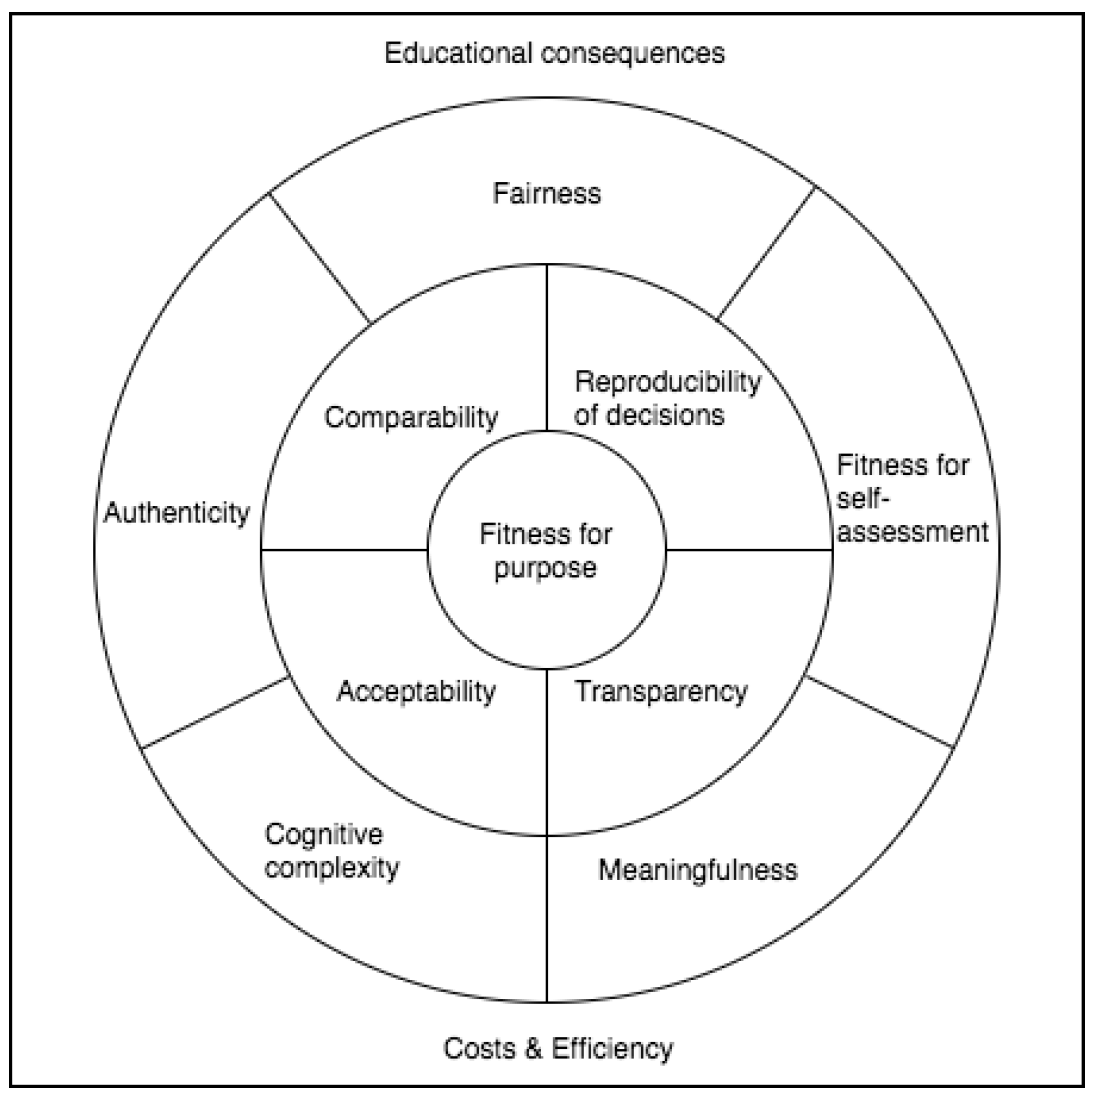
\includegraphics[scale=0.6]{figures/AdaptedQualityCriteriaCatete.png}
\caption{The Wheel of Competency Assessment (2017Catete)}\label{fig:AdaptedQualityCriteriaCatete}
\end{figure*}



\subsubsection*{Design methods}
The Dutch curriculum description includes high-level goals (\cite{Barendsen2016}). This description is not specific enough for creating assessment tasks. For alignment, concrete learning outcomes and specified level of comprehension (taxonomy) need to be established (\cite{biggs1996}). A similar situation exists in the UK national curriculum. The levels from the previous ICT curriculum have been removed, leaving assessment at KS3 to the responsibility of individual schools. CAS members (in co-operation with CAS Master teachers, teachers and academics) have taken the initiative to establish computing progression pathways and rubrics to assess learners' Problem-solving and Computational Thinking capabilities (Dorling and Walker, 2014).
Their work is based on the CT definition from the CSTA five dispositions/attitudes and builds on the work of Brennan and Resnick (2012). With it, learning objectives and potential evidence observations have been established. However, there is no indication of concrete alignment with assessment tasks. Importantly, Giordano et al. \cite{Giordano2015} concludes that designing questions which are clearly linked to the competencies is perceived as the most difficult task in the assessment process. Moreover, the more authentic and realistic, the more complex the detailed mapping to the abilities/competenties becomes. This is very relevant, as the curriculum specifies a concept-context approach to learning (\cite{Barendsen2016}). This authentic learning approach encourages students to connect real world problems to the subject matter at hand. In their paper, Goode et al. (\cite{goode2014curriculum} emphasize why this makes sense: "engaging students in the context of complex, meaningful projects that require sustained engagement, critical thinking, collaboration, management, communication, and management of resources to develop final products or presentations builds the types of 21st century skills advocated by new sets of national standards". Especially when dealing with more complex tasks, to ensure a valid assessment, explicit alignment between learning objectives, specifications of which evidence infers the attainment of an objective, and tasks to evoke this evidence must be established.


In his work, Hermansen (\cite{hermansen2014reworking} suggests that teachers should work collaboratively on transforming (rather than implementing) assessment tasks. Such a development and refining process yields assessments specific to local settings, adhering to the needs, knowledge, skills and interests of their own students. Customizing assessment to specific local settings is a key issue. Firstly, it supports pedagogical link-making described by Scott et al. (\cite{scott2011pedagogical}) as being fundamental to science learning. Secondly, it fits in seamlessly with an authentic concept-context approach where the assessment is to be modified according to the chosen context.
%bare necessity for implementing a concept-context approach.


%\subsubsection*{Learning objectives and KSAs}
\todo{ Naar achtergrond met meer toelichting, uitleggen. What is abilities (niet attitutes?)? What is verschil tussen skill en abilities?}
\todo{Why needed}


\note{knowledge, skills or other attributes}
%
%linked to evidence-eliciting-performances



\textbf{Evidence-Centered Design}\newline
Initiatives in the U.S. follow a structured path, incorporating validity evidence into an assessment design process. SRI launched a Teacher Assessment Literacy for Exploring Computer Science study to investigate the design and delivery of high-quality assessment literacy materials. They apply the Evidence-Centered Design (ECD) method. ECD is a principled method for modeling domains for assessment purposes that is especially useful for hard-to-assess practices (\cite{grover2016assessing}). Figure \ref{fig:ECD} gives an overview of the processes and products of each of the five ECD layers. ECD's systematic structure facilitates a coherent mapping from high-level curricular goals to observable behaviors. This yields three models designed to elicit evidence of students' achievement levels of the relevant learning objectives. The student model specifies the knowledge, skills or other attributes (KSA) to be assessed. The evidence model describes observable behaviors or performances which may provide evidence about the KSAs, and thus links the chain of reasoning from students’ performances to their knowledge and skills. The task model describes the environment in which students say, do, or make something to provide evidence. Evidence is obtained by deliberately putting students in those situations, challenges, or tasks that will elicit the desired KSAs (Grover and Bienkowski, forthcoming). Mislevy's 2006 (\cite{mislevy2006implications}) report on the application of this method has received many citations. This methodology has recently been used in CS by Grover (\cite{grover2017measuring}) to assess problem-solving processes, and for the development of assessment instruments for the Exploring Computer Science curriculum by McGee (\cite{McGee2018ECS}) and by Rutsein, Snow and Bienkowski (\cite{rutstein2014computational}\cite{snow2017CTECD})\todo{for AP CS Principles}\todo{[2018McGee CS outcomes]}





\note{Evidence models
lay out the argument about why and how observations in a given task
situation constitute evidence about student model variables. There are
two parts to an evidence model, the evaluation component and the
measurement component.}

%This methodology has been used by, extensively reported on, and cited to by Mislevy et al. (2002, 2003).




\begin{figure*}
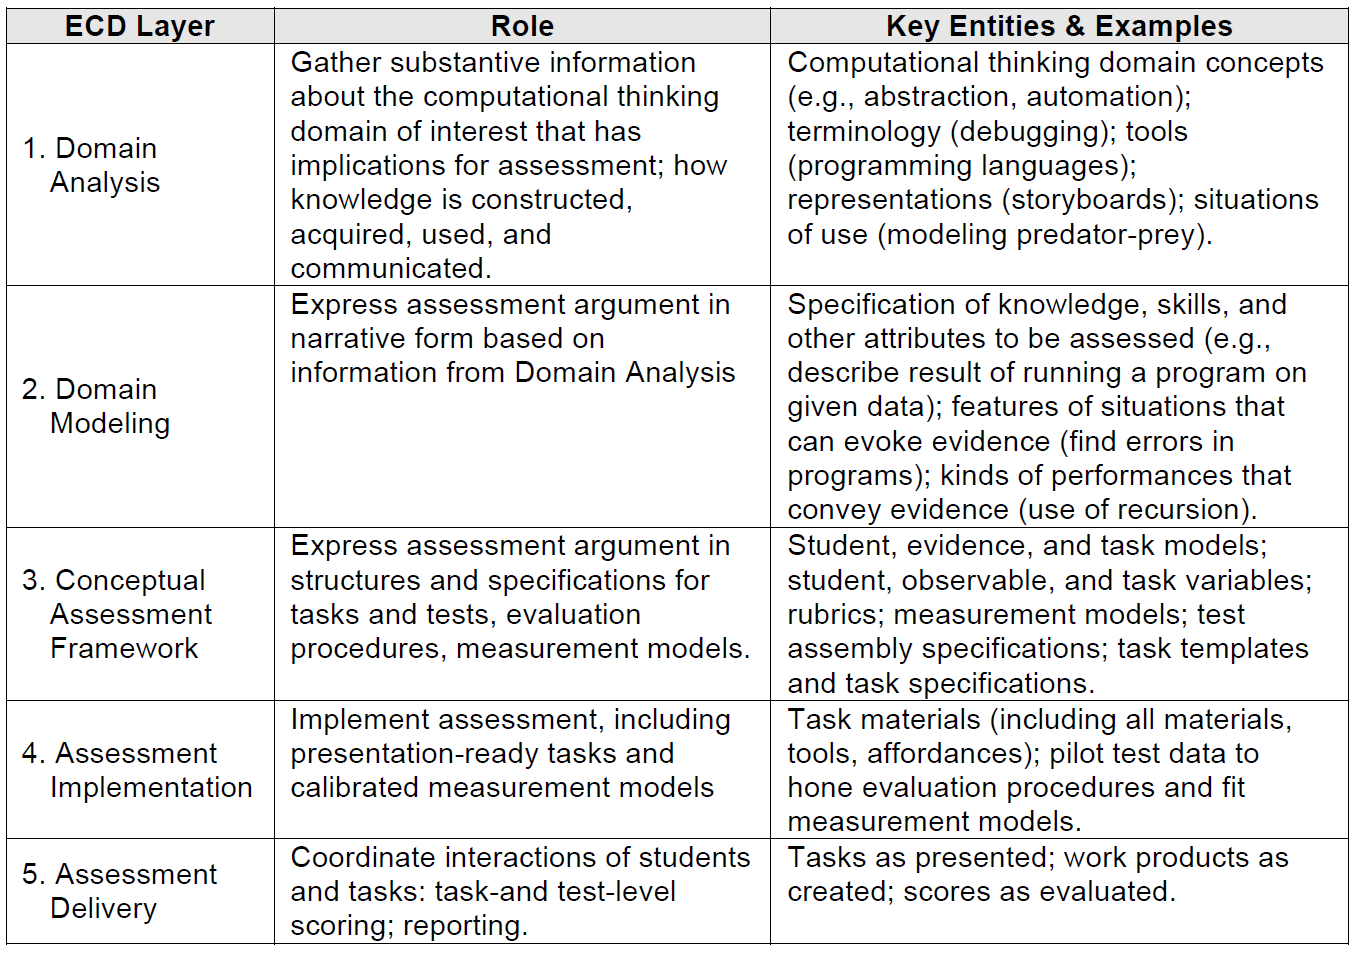
\includegraphics[scale=0.8]{figures/ECDoverview.png}
\caption{Roles and Key Entities in the Five Layers of Evidence-Centered Design (2014SnowBienkowski)}\label{fig:ECD}
\end{figure*}



%\begin{itemize}
%\item \textbf{Domain Analysis:}
%The top layer in the ECD process is a Domain Analysis to clarify learning goals.
%This level includes determining relevant concepts and terminology,(e.g. abstraction, algorithms), tools (i.e. programming languages) and representations (flowcharts, pseudocode) as well as understanding how knowledge is constructed, acquired, used and communicated (SRI Assessment Design Patterns for CT, 2017). In the process, the curricular learning objectives are translated into more specific and learning goals specified in operational terms, ready for teacher use
%\item \textbf{Domain Modelling:} the assessment argument was designed. The learning goals were translated into the specific focal knowledge, skills, and attributes (KSAs)
%
%\item \textbf{Conceptual Assessment Framework:}
%The result of this phase was a design pattern consisting of three aligned models (student model, evidence model, and task model) which together form the assessment specifications: the foundation for the new assessment.
%
%\item \textbf{Assessment Implementation:}During the implementation stage, the model assessment tasks are translated into classroom-specific assessment tasks in the designated programming language.
%
%\item \textbf{Assessment Delivery:} the tasks are administered to students.
%\end{itemize}


Transitioning from one ECD layer to the next involves analytical precision and careful reasoning. To validate this step, Catete (2017) uses an expert panel. Several methods can be used to resolve differences in opinions and obtain an objective consensus between panel members, such as focus groups\todo{ref WIPSCE artikel over thresholds}, Nominal Group Technique\todo{Adler, M. and Ziglio, E. Gazing into the oracle: The Delphi method and its application to social policy and public health. Jessica Kingsley Publishers, 1996.} or the Delphi method\todo{ref brooks 779}.

The purpose of the Delphi technique is to test opinion consensus amongst a group of experts. It is usually employed in research where there is a high level of uncertainty or the collective opinion of
experts would be beneficial (2017Kallia). Using this technique, a group of experts is brought together (either virtually or physically) to answer a question. After the first round, the participants' responses are shared anonymously, and the question is re-stated. This process repeats until a consensus is reached. In his study on consensus methods, Vernon (2009Vernon) states that consensus values lie between 55\% and 100\%, and modus 70\%.

\todo{Methode geven om meningsverschillen plat te strijken.  DELPHI?? De moeite waard? Misschien delen van DELPHI methode gebruiken? Kijk evt naar artikel over thresholds WIPSCE, evt met een focusgroep (is sneller en minder zwaar aangezet). Beschrijf hier hoe je verschillen gaat oplossen. Relateer evt ook aan ECS ECD met DELPHI. Elementen van methode gebruiken, niet hele methode, Nominal Group Technique? (zie 2017 catete.}

\todo{Kallia, Sentance WIpsce 2017 Computing Teachers' Perspectives on Threshold Concepts describe and use the delphi method}



\subsubsection*{Taxonomies}

Taxonomies provide a language for describing learning outcomes and
performance in assessments, dividing them into domains (such as cognitive, affective, and psychomotor) or categories based on complexity of the task. Two widely used taxonomies for assessment of learning are the (revised) Bloom
taxonomy and the SOLO taxonomy. Both have been used in CS education research, for example, the revised Bloom by Whalley et al. (\cite{Whalley2006}) and SOLO by Lister et al. (\cite{lister2006not}\cite{lister2010naturally}).

\textbf{Bloom's Taxonomy}\newline
Bloom's taxonomy was designed to make assessment more systematic, by distinguishing between different types of learning objectives (from understanding to creating) and across multiple domains of learning (factual, conceptual, procedural, and metacognitive). Figure \ref{fig:BloomsRevised} depicts the hierarchy of the types of learning objectives.


\begin{figure*}
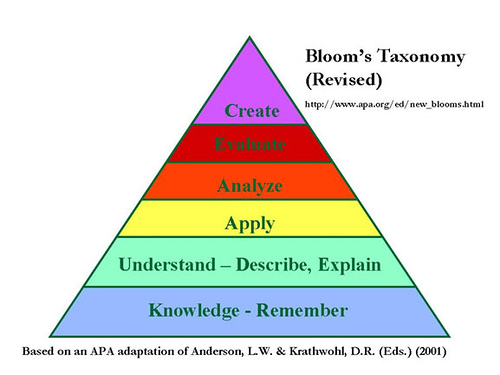
\includegraphics[scale=0.6]{figures/bloomsrevised.jpg}
\caption{Revised Bloom's Taxonomy (2002Krathwohl)}\label{fig:BloomsRevised}
\end{figure*}


Drawbacks to the use of Bloom's taxonomy in CS have been reported. Thompson et al. (\cite{thompson2008bloom}) conclude that experts have difficulties applying Bloom's taxonomy consistently in introductory programming courses. Meerbaum-Salant et al. (\cite{Meerbaum2013}) similarly report issues with classification, and relate them specifically to the nature of the tasks. Whalley et al. (\cite{Whalley2006}) express that it is helpful for generating example tasks, but had difficulty placing then within the revised taxonomy. As a result, all comprehension (reading) questions were categorized into one and the same level: Understanding. The classification becomes meaningless if every task, irrespective of its complexity, falls into the same category.


\textbf{Solo's Taxonomy}\newline
Biggs (\cite{biggs1996}) proposes the Structure of the Observed Learning Outcome (SOLO) taxonomy, which classifies learning outcomes in terms of their complexity. The SOLO taxonomy differentiates between a local and a holistic perspective. Understanding can reside along the following scale, from prestructural (incompetence), unistructural (able to identify one relevant aspect), multistructural (able to combine several relevant but independent aspects), relational (able to analyse or apply that what is integrated into a structure) to extended abstract (being able to generalize to a new domain). As such, the scale can be used to discriminate between being able to read code line-by-line (but not understanding its purposeful intent) from fully understanding and summarizing the goal of a piece of code as an entity. Though SOLO can be used for holistic marking, it says nothing about the type cognitive processing, such as recalling items or drawing conclusions (\cite{Fuller2007}).


Given the difficulties in categorizing programming activities within the existing taxonomies, several attempts have been made to propose new taxonomies which may be more appropriate for CS education. Fuller et al. (\cite{Fuller2007}) suggest to separate Bloom’s levels into two dimensions, producing (writing) and interpreting. Lister and Leaney (\cite{lister2003}) attempt to differentiate in terms of magnitude of the code (i.e. number of lines of code). Lister et al. (\cite{lister2010naturally}) propose a refinement of the SOLO taxonomy to account for both the practical and conceptual learning goals in CS. For example, they propose and extension of the taxonomy to code-writing questions by considering a degree of 'partial correctness'.


Meerbaum-Salant et al. (\cite{Meerbaum2013}) propose a hierarchical taxonomy scale describing how student’s performance grows in complexity. It’s aim is to pinpoint (the development of) programming skills: both problem solving (such as plan composition) and (construct-based) language aspects. It is based on a combination of the Revised Bloom and Solo taxonomies. The result is a nine-level taxonomy with
the highest level being relational creating, and the lowest level being
unistructural understanding (on one axis: understanding, applying, creating; on the other: unistructural, multistructural, relational):


%Meerbaum-Salant et al. (2013) propose a hierarchical taxonomy
%scale based on a combination of the revised Bloom and Solo taxonomies
%\cite{Meerbaum2013}. Three super-categories - unistructural, multistructural,
%and relational (derived from the Solo taxonomy) were chosen, each containing
%three sub-categories - understanding, applying, and creating (derived from
%the revised Bloom's taxonomy:

\begin{description}[leftmargin=1em]
\item[Understanding:] The ability to summarize, explain, exemplify,
    classify, and compare CS concepts, including programming constructs.
\item[Applying:] The ability to execute programs or algorithms, to track
    them, and to recognize their goals.
\item[Creating:] The ability to plan and produce programs or algorithms
    (constructing, analysing, evaluating and formulating).
\item[Unistructural:] The ability to create very small scripts doing one
    thing, or adding an instruction with a local effect to an existing
    script.
\item[Multistructural:] The ability to track a program and grasp various
    parts but not the entity they form as a whole.
\item[Relational:] The ability to fully understand a complex concept (such
    as concurrency) and to coherently explain its various facets.
\end{description}



Though the proposed taxonomies have their differences, they all consider two important coding aspects: reading versus writing, and the complexity of the problem.

For the assessment of CT, Zhong et al. (\cite{Zhong2016}) propose a three-dimensional framework, adapted from Brennan and Renick (\cite{BrennanResnick2012}), and extend it with attributes for computational concepts, computational practices and computational perspectives.


\subsubsection*{Progression Pathways}



In his work, Lister (\cite{lister2010naturally}, \cite{lister2016toward}) positions the Piagetian and neo-Piagetian theories. The Piagetian theory describes how students may reside in different stages of cognitive development for each fundamental concept being taught: pre-operational, concrete operations, and formal operational. The neo-Piagetian theory extends this with the idea with an ”overlapping waves” model, a novice programmer can reside in multiple stages simultaneously. The stages coincide with those of the SOLO taxonomy. In their paper, Szabo et al. (\cite{szabo2014neo}) propose a curriculum analysis methodology based on Neo-Piagetian theory to facilitate lecturers in tracing the development and assessment of concepts throughout their courses. This theory describes how students may reside in a different stages of cognitive development for each fundamental concept being taught.

Denning \cite{denning2017remaining} calls competency tests which are supported by guidelines for different skill levels of CT. Similar to the neo-Piagetian stages (pre-operational, concrete operations, and formal operational)(\cite{szabo2014neo}), he uses Dreyfus' model of progression from beginner, advanced beginner, competent, proficient, expert, through to master.

CAS has made a start (work in progress) by establishing Computing Progression Pathways (\cite{Dorling2014CTprogressions}) to identify the major knowledge areas (concepts) and CT skills of computing and provides specific indicators of increasing levels of mastery (e.g. distinguishing between ‘understands’ and ‘can apply’) of the subject in those areas (\cite{Giordano2015}). However, the framework does not discuss abilities to be acquired\cite{denning2017remaining}.



\todo{ Erik: Licht toe en zet tegen elkaar af: “de ene onderzoek maakt wel onderscheid tussen verschillende… maar niet…”} \todo{ Nesten is een complexiteit op zichzelf
“Afhankelijkheid is geen onderdeel van de onderzoek van… “}

\begin{figure*}
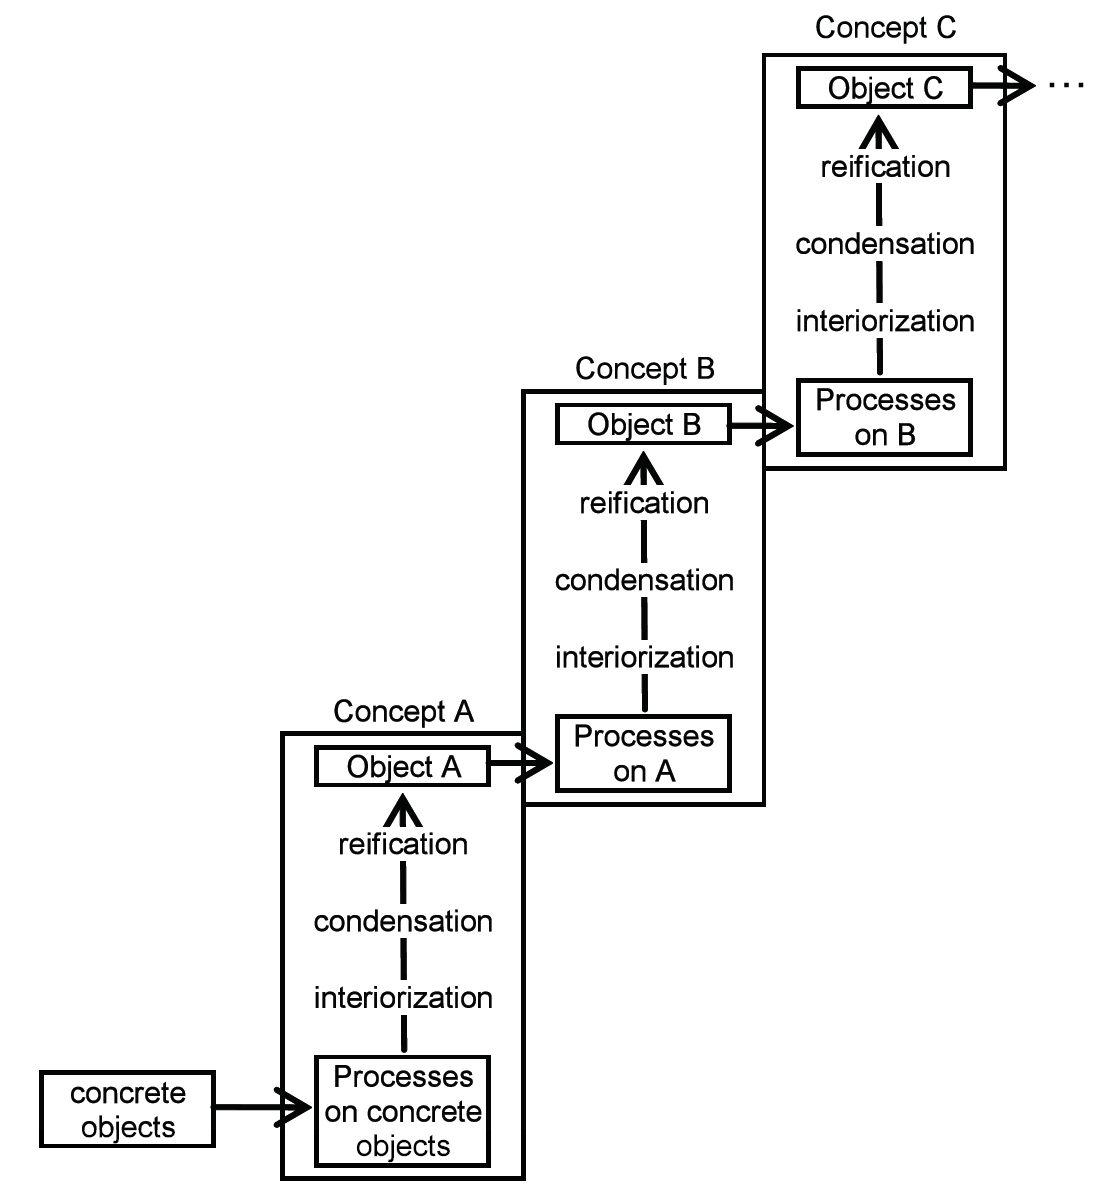
\includegraphics[scale=0.8]{figures/ListerFases.png}
\caption{General model of concept formation (2010Lister), after Sfard (1991)}\label{fig:ListerFases}
\end{figure*}

In their work, Lister et al. (\cite{lister2004multi}) describe transition between different levels to take place on a concept-by-concept basis. Thus, whilst a student resides on a certain level for a particular concept, the same student could have a complete other level of understanding for another concept. See figure \ref{fig:ListerFases}.





Misconceptions on a particular concept may lead to problems when learning other concepts for which that concept knowledge is pre-requisite. It is thus important to identify the level of understanding per individual concept.



\subsubsection*{Identifying levels of mastery}
Assessment tasks should adequately indicate a students’ programming comprehension and clearly discriminate between achieved performance levels. Predicting the difficulty of programming tasks and understanding alternative conceptions has shown to be difficult (\cite{Lonati2017Bebras})\todo{ Toelichten: bv een invulopgave kan op verschillende manieren aangepakt worden}.


A substantial body of work has previously explored the assessments used in novice programming courses in tertiary education (Luxton-Reilly, 2018)\todo{mer woorden gebruiken, uitleg vanuit docenten stoel}. In prior work, researchers claimed that the subject itself was difficult. McCracken et al. (\cite{McCracken2001}) discuss how students fail to complete tasks, and Robins, Rountree, Rountre (\cite{robins2003learning}) associate it with high dropout rates in introductory programming courses. Using the work of Lister et al. (\cite{lister2004multi}) as a starting point, the "Leeds" ITiCSE working group inferred that students lacked basic skills pre-requisite for problem-solving, such as reading program code. More recently, assessment tasks were found to be more complex than academics expected (\cite{LuxtonReilly2018}). For example, tasks typically require both algorithmic thinking (initialize before changing), as well as a more advanced understanding of data representation (assigning a value to a property)(\cite{Seiter2013}). In their research Luxton-Reilly (\cite{LuxtonReilly2018}) state that “most assessments used in formal examinations combine numerous heterogeneous concepts, resulting in complex and difficult tasks”.

However, whatever taxonomy chosen, scientists agree that classifying tasks is far from straightforward (\cite{Fuller2007}, \cite{thompson2008bloom}, \cite{LuxtonReilly2018}, \cite{Whalley2006}, Hu, and Robbins, 2008). As a result, researchers exclaim that "the pattern of achievement is not clear" (\cite{ZurBargury2013}), making analysis difficult and inconclusive. Maybe the issue is not the taxonomy, but rather the task being classified?


In their findings, Oliver et al., (2004) indicate that introductory and intermediate programming courses assess at a constant level of difficulty and restricted solely to Bloom’s application and analysis level. The inability to accurately measure student performance may well contribute more to the poor results highlighted in several studies (such as the McCracken et al. \cite{McCracken2001}) than failures of student comprehension \cite{2010TewGuzdial}.  In their paper, Whalley et al. (\cite{Whalley2006}) also relate the high failure rate in introductory programming courses to unfair and inappropriate assessment instruments, and express that this may be especially true for non-elite institutions where less expertise is available.


In their combined efforts, Luxton-Reilly et al. (\cite{LuxtonReilly2018}) have managed a first step towards decomposition, by for example recognizing and identifying initialization, use of conditionals and nesting. They use a top-down approach in which they decompose a complex task into its constituent concepts. However, such a top-down approach does not consider all concept combinations, and therefore may omit sources of difficulties and alternative conceptions. For example, in their nesting-task, a student may not understand the difference between a loop nested in a conditional and a conditional nested in a loop.



De Raadt et al. (\cite{deRaadt2009teachingPlans}) describe a set of elementary plans (programming strategies) that can be combined to create a solution. Examples of elementary plans are Initialization plan (variables), Average plan, Triangular Swap plan, Guarded Division plan, Counter-Controlled Loop plan, Sum and Count plans, Bubble Sort algorithm. They explain that the identification, selection and application of plans can be seen as a representation for strategy (similarly described by Soloway (1985), also known as patterns (Wallingford, 1996)) and should be taught and assessed explicitly.
Strategies can be expressed both simply, at a sub-algorithmic level, and at a higher level which are found in solutions produced by expert programs (\cite{deRaadt2006}). \todo{A number of attempts have been made to decompose these strategies (Muller, Haberman, and Ginat, 2007; Porter and Calder, 2003; Wallingford, 2007)} \todo{ Erik: uitsplitsen en toelichten wat ieder gedaan heeft zodat je dit als lezer niet zelf hoeft op te zoeken }into  smaller units and distinguish pre-requisite knowledge. These plans and higher level algorithms map to multi-structural and relational levels in the SOLO taxonomy. Soloway (p. 856) and de Raadt identify the following methods of integrating plans (bottom-up):
\begin{itemize}
\item Abutment: plans following each other in sequence. For example, initializing a variable and printing it’s value. For example:
\begin{verbatim}
x=12
print("The value of x is: ", + str(x) )
\end{verbatim}

\item Nesting: one plan as a whole is submerged in another. For example, printing the value of a variable during intermediate iterations of a counting plan. For example:
\begin{verbatim}
counter=0
while not done():
    counter+=1
    print("The number of items is: " + str(counter))
\end{verbatim}

\item Merging: interleaving (at least) two plans. For example, in the averaging problem, the input, summing and counting plans are merged.
\end{itemize}

De Raadt et al.'s research is not directly applicable to secondary education. Underlying concepts at a basic unistructural level which may assumed to be trivial (at CS1 level), may not be so trivial at all in secondary education. For example, the 'average plan', explicitly states the need to understand the division operator, but doesn't say anything about pre-requisite knowledge about the assignment of variables. Other concepts which are (explicitly or implicitly) stated in reformed CS curricula but not included in the plans are: procedures, functions, parameters, and a Boolean-Flag loop plan as a specific form of a primed sentinel controlled loop plan. Misconceptions about these concepts has been researched and documented, for example by Sorva (\cite{sorva2013notional}) and \url{PD4CS.org}.



\subsection*{PCK}

Effective teaching requires a combination of pedagogy, content, and knowledge (PCK) (\cite{shulman1986pedagogical}). In their PCK based research, Yadav et al. (\cite{Yadav2016}) interviewed high school teachers in the U.S. to understand the challenges they face.

In a nutshell, PCK means that subject matter (content knowledge) and ways of teaching (pedagogical knowledge) are integrated(\cite{Yadav2016}). It encompasses knowing what makes certain topics easy or difficult, as well as ways of representing and formulating topics in different ways (\cite{shulman1986pedagogical}). In their paper, Kao et. al. (\cite{Kao2018}) propose and piloted a 9 question pre-test and post-test to assess different aspects of CS PCK amongst pre-AP and AP CS teachers. They specified several important CS PCK characteristics, particularly teachers' knowledge of explanations, suboptimal solutions, and misconceptions.

Yadav et al. \cite{yadav2014computational} piloted a module to teach CT to pre-service teachers and concluded that it was effective in influencing teacher's understanding and positive attitude toward CT and its integration into the classroom. Teaching PCK can be effective.





Magnusson, Krajcik en Borko (1999) distinguish four aspects of content-specific PCK: knowledge of
(1) curricula, (2) students' understanding and difficulties, (3) instructional strategies, and (4) assessment.


In this research we focus on just one aspect of PCK, namely (4) assessment. We are particularly interested in the PCK aspects needed to adapt and implement particular types of assessment, those that elicit algorithmic thinking.


\subsubsection*{Assessment as a part of PCK}
Very little is known about PCK for Computing (\cite{Yadav2016}). As a part of PCK, teachers have limited knowledge about assessment and seriously struggle with it (Popham, 2009). Particularly, teachers face many challenges with respect to the assessment of new topics (DeLuca and Klinger, 2010). The 2015 study by Computer Science Teacher's Association (CSTA) found that teachers face a number of challenges finding valid and reliable assessments to use in their classrooms. Along the same line, Dutch teachers say they lack qualitative (peer-)reviewed materials, assessment rubrics and question banks (\cite{tolboom2014informatica}). Yadav et al. (\cite{Yadav2015}) conclude that teachers lack PCK, which manifests itself in an incapacity to act: teachers understand need for qualitative assessment, but just don't know how to.

%Both experienced and novice teachers struggle in assessing student learning (Fincher, Kolling, Utting, %Brown, Stevens 2010)(Hebert \& Worthy, 2001)(Veenman, 1984) (Yadav, 2016)(Yadav, %2015)(Bardensen et al., 2015 ITICSE wg).

Faced with a specific assessment task, teachers generally take previously developed templates as a point of departure and adapt them to meet their current requirements (\cite{hermansen2014reworking}). During his observations he saw that teachers spent significant time on aspects related to eliciting evidence of students' approach to a task. This indicates that teachers are well-informed about the role of an assessment.
Particularly, teachers face many challenges with respect to the assessment of new topics (DeLuca and Klinger, 2010). The 2015 study by Computer Science Teacher's Association (CSTA) found that teachers face a number of challenges finding valid and reliable assessments to use in their classrooms. Along the same line, Dutch teachers say they lack qualitative (peer-)reviewed materials, assessment rubrics and question banks (\cite{tolboom2014informatica}). Yadav et al. (\cite{Yadav2015}) conclude that teachers lack PCK, which manifests itself in an incapacity to act: teachers understand need for qualitative assessment, but just don't know how to. To elicit: CS teachers assess merely a small spectrum of levels in Bloom's taxonomy, ascertained by Oliver et al. (\cite{Oliver2004}) and confirmed by Whalley et al. (\cite{Whalley2006}). Depending on the particular concept, in some cases only the lower knowledge levels are assessed (networks), in others predominantly the higher application and analysis levels (programming). Either way, this leads to non-discriminative assessments. Even if there is published material available, many teachers create and rely on their own material (\cite{popham2009assessment}).

Thus, judgements about students' proficiency are made without the use of validated, sometimes not even valid assessments. Whalley et al., (\cite{Whalley2006}) describe the assessment of programming as complex and challenging and emphasize the lack of clear frameworks and tools. This is alarming. Ragonis (\cite{ragonis2012type}) states that if the quality of assessment is insufficient, teaching will be ineffective.  Giordano et al. (\cite{Giordano2015}) add that if teachers use low-quality assessment instruments we will end-up teaching the wrong subject, and vice-versa.


In his review on developing generic resources for assessment, Hermansen (\cite{hermansen2014reworking}4) concludes, based on several researches (Coburn, 2001, 2003; Edwards, 2008; Horn \& Little, 2010; Hutchinson \& Hayward, 2005; Rasmussen \& Ludvigsen, 2009; Tierney, 2006), that assessment tools aren't plug-and-play modules that can be relocated and implemented as-is. Rather, in order to remain operable they must be adapted and 'recontextualized' according to classroom needs. From his extensive literature review ((Black \& Wiliam, 2006; Brookhart, Moss, \& Long, 2010; Harrison, 2005; James \& Pedder, 2006; MacPhail \& Halbert, 2010; Suurtamm et al., 2010; Webb \& Jones, 2009; Willis, 2011) Hermansen summarizes that teachers who implement formative assessment resources "draw upon a strong understanding of subject knowledge, use a range of ideas and tools to enable classroom interaction and learning, have established a new division of labour in their classrooms, focus on developing student learning and autonomy, and critically examine their own beliefs about learning and classroom practices". This list alone affirms that any teacher new to teaching, or new to a particular concept, will likely be lacking some, if not all of these skills or knowledge.


Teacher educators need to provide teachers with the content, pedagogy, and instructional strategies needed to incorporate computational thinking, and in particular the assessment of the its core concepts (\cite{Yadav2017CTteacherEd}).



\subsubsection*{Assessing CT}
With the lack of a precise definition as one of its contributing factors, Computational Thinking is perceived to be one of the more challenging concepts to teach and assess (\cite{crick2017}).

There is no clear definition of CT(Crick, 2017) making it difficult to assess. Recently some research into assessment of Computational Thinking has been published (\cite{Yadav2017CTteacherEd},\cite{Yadav2016}). Evaluating CT is perceived as difficult (Brennan and Resnick, 2012) (Crick, 2017).
Without rigorous assessment, computational thinking cannot be successfully embedded in education (Grover et al., 2014).

Grover et al. (2017) call for measures that enable educators to assess student learning of CT.  Specifically they signal the necessity to test and validate materials in various settings with diverse learners.
Assessments of CT remain underdeveloped and under-researched (\cite{Yadav2015}).
Educators need a manner to assess and validate what CT a student has learned (\cite{GroverPea2013}).
In their review study, Lye and Koh\cite{LyeKoh2014}, summarize that of the research on computational thinking through programming , stunningly none focus on upper secondary high school (ages 15-18) (but merely on elementary or higher education).


\subsubsection*{Assessing Algorithms through programming}
Traditionally, assessment of algorithms takes place through programming: reading or writing code.

The 2001 ITiCSE report by the McCracken Group (\cite{McCracken2001}), a keystone in assessment literature (\cite{Giordano2015}) on CS concepts, describes the difficulties pertaining to the development and validation of assessment activities. They raise concerns about task selection and the difficulties of standardizing assessments for multiple institutes. According to Snow (\cite{snow2017CTECD}), the higher CS education community has made an effort to create programming language-independent assessments, which are in various stages of being evaluated. The primary goal here is to establish tasks that can be used at multiple institutions. In their research, Whalley et al. (\cite{Whalley2006}) noted, while translating questions from one language to another, that unique idiomatic and syntactical features may have effect on the appropriate choice of distracters (i.e. subtle differences in initialization values for indexes and in relational operators).

From the new CT viewpoint, algorithms can also be articulated and assessed without involving programming. The output could be a flowchart \cite{Smetsers2017} or pseudocode. For example, Tew and Guzdial (\cite{2010TewGuzdial}) choose for a wordy pseudocode to create assessments independent of a programming language.


\subsubsection*{Fit-for-purpose assessment tasks}
There has been quite some research done on the effectiveness of different types of assessments, each with its own advantages and disadvantages. Brennan and Resnick (2012) use multiple approaches to assess student's learning. In their research, Grover (2017) argue for a multi-facetted assessment. Due to the both the cognitive and non-cognitive aspects of learning CT, multiple measures contribute to an accurate picture of the students capabilities. There is also quite some research done on (CT) competitions, such as Bebras (Dagiene and Sentance, 2016) and Informatics Olympiads (2017Lonati).


Gathering evidence of task performance can take many forms: written examens, open-ended projects, analysis of digital artifacts (\cite{BrennanResnick2012}, 2012), artifact-based interviews (Grover et al., 2015), game design tasks (\cite{snow2017CTECD}).


Projects can be in multiple forms, charettes (fixed-length laboratory assignments) or across an entire course. It's result can be a written report, a digital artifact, comments in code, presentation, logbook, project notes or combination of one or more of these. Evidence can be based on real-time observations.

According to the description of open and semi-open tasks used by Zhong et al. (2016), a mapping to multi-structural and relational cognitive levels on the SOLO taxonomy seems plausible, whereas the closed tasks reside on a unistructural level. Thompson (2016) looked at "explain in plain English" tasks and conclude that despite that they may be ambiguous, they are a reliable indicator of a student’s ability to respond relationally.


Written examen themselves can have tasks of different nature. Lister et al. (2010) summarize a list, including debugging, tracing modifying question. An interesting task is a Parson's Problem. The correct lines of code are provided in random order, and must be rearranged correctly. Whilst lowering the cognitive load, Parsons problems can be used to focus assessment specifically on misconceptions or areas that learners typically struggle, and their difficulty is easily adapted (2017EricsonParson).

Atmazidou (2016) uses self-reflection to assess the different aspects of computational thinking.

courses are multiple choice tests. According to Tew and Guzdial (2010) when constructed carefully, they can provide the same information about conceptual knowledge as short answer or open response questions with significant advantages in test administration and scoring. Morrison and Free (2001) explain that they can also be used to assess higher-order thinking. And indeed, they appear in AP CS Principle exams to assess computational thinking skills. However, distractors must be selected carefully.

%CS1 much research to assessment tasks: mc, parsons, sniplets,
%meet the criteria in \ref{sec:qualityCriteria} in addition

For the open tasks Zhong et al. (Zhong2016) used project evaluation as a means of summative assessment, and reflection report and creative design report as a means to evaluate the process.




\subsection{The Black hole: Assessment in Secondary CS education}
There is a gap between the (lean) research and classroom practice (\cite{Yadav2015}). All-in-all, little research has been done on the effectiveness of the assessment materials available (\cite{Yadav2016}). Computing education and research suffer from the lack of assessment instruments (\cite{voogt2017effecten}. In their research Tew and Guzdial (\cite{2010TewGuzdial}), argument the importance of validated assessment that could be widely applicable across tertiary curricular approaches. This may be even more true for secondary education, where far less relevant research has been done in the first place. In addition, research developments are not accessible to teachers (either they need a paid subscription, academic literature may be written in an incomprehensible manner, or not practical as it can’t be implemented in the classroom in a cost-effective manner). Recent published work based on CT have a focus in primary education or middle school (\cite{LyeKoh2014}). Research based on (the assessment of) CS concepts has a focus on tertiary education (such as \cite{McCracken2001},\cite{2010TewGuzdial}). Merely a few studies focus on CS concepts or CT specifically in secondary education.




Summarizing, the introduction of the new computing curriculum could benefit from tooling which supports the creation of qualitative knowledge and competency based assessments. Teachers will and should create assessments tailored specifically to their classroom needs, but lack specific PCK to do so. Not only is creating a qualitative assessment acknowledged as a difficult task, in the current situation, teachers must first acquire and internalize knowledge about the new concepts.
